%%%%%%%%%%%%%%%%%%%%%%%%%%%%%%%%%%%%%%%%%%%%%%%%%%%%%%%%%%%%%%%%%%%%%%%%%%%%%%%%%%%%%%%%%%%%%%%%%%%%%%%%%%%%%%%%%%%%%%
\chapter{Results for non separable $p$} \label{sec:para}%%%%%%%%%%%%%%%%%%%%%%%%%%%%%%%%%%%%%%%%%%%%%%%%%%%%%%%%%%%%%
%%%%%%%%%%%%%%%%%%%%%%%%%%%%%%%%%%%%%%%%%%%%%%%%%%%%%%%%%%%%%%%%%%%%%%%%%%%%%%%%%%%%%%%%%%%%%%%%%%%%%%%%%%%%%%%%%%%%%%
We will now try to use what we learned from the previous section in a parallel setting with $p$ non separable and see if we can make KPM outperform DM.
We start by showing convergence in section \ref{sec:pconv}, and proceed with looking into speedup and parallel efficiency in section \ref{sec:speed}. We end by investigating how computation time for the best possible case of KPM compares to DM, in section \ref{sec:compare}. 

%%%%%%%%%%%%%%%%%%%%%%%%%%%%%%%%%%%%%%%%%%%%%%%%%%%%%%%%%%%%%%%%%%%%%%%%%%%%%%%%%%%%%%%%%%%%%%%%%%%%%%%%%%%%%%%%%%%%%%
\section{Convergence} \label{sec:pconv}
%%%%%%%%%%%%%%%%%%%%%%%%%%%%%%%%%%%%%%%%%%%%%%%%%%%%%%%%%%%%%%%%%%%%%%%%%%%%%%%%%%%%%%%%%%%%%%%%%%%%%%%%%%%%%%%%%%%%%%
\begin{figure}[H]
        \centering
        \begin{subfigure}[b]{0.45\textwidth}
                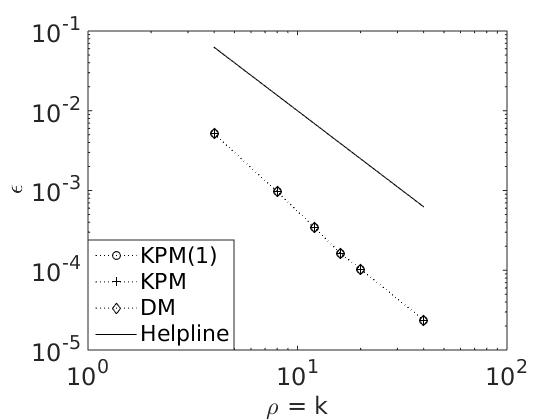
\includegraphics[width=\textwidth]{fig/p1conv1}
                %\includegraphics[width=\textwidth]{test}
                \caption{function \texttt{P1}}
                \label{fig:conv1p}
        \end{subfigure}%
        ~
        \begin{subfigure}[b]{0.45\textwidth}
                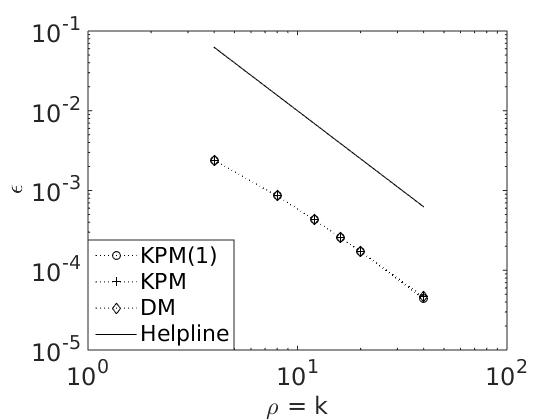
\includegraphics[width=\textwidth]{fig/p2conv2}
                %\includegraphics[width=\textwidth]{test}
                \caption{function \texttt{P3}}
                \label{fig:conv2p}
        \end{subfigure}
        \caption{A convergence plot for several methods with $\rho = k$. The helpline shows quadratic convergence.}\label{fig:convp}
\end{figure}
As can be seen from figure \ref{fig:convp}, all methods converges quadratically and identically, as in section \ref{sec:sconv}. All methods therefore perform as expected regarding convergence.
%%%%%%%%%%%%%%%%%%%%%%%%%%%%%%%%%%%%%%%%%%%%%%%%%%%%%%%%%%%%%%%%%%%%%%%%%%%%%%%%%%%%%%%%%%%%%%%%%%%%%%%%%%%%%%%%%%%%%%
\section{Speedup} \label{sec:speed}
%%%%%%%%%%%%%%%%%%%%%%%%%%%%%%%%%%%%%%%%%%%%%%%%%%%%%%%%%%%%%%%%%%%%%%%%%%%%%%%%%%%%%%%%%%%%%%%%%%%%%%%%%%%%%%%%%%%%%%
\begin{figure}[H]
        \centering
        \begin{subfigure}[b]{0.45\textwidth}
                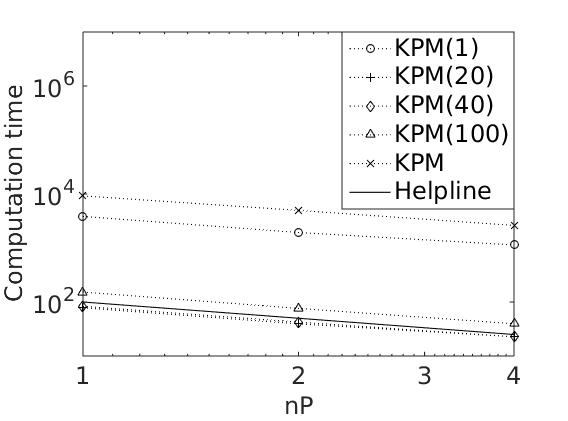
\includegraphics[width=\textwidth]{fig/u1para1}
                %\includegraphics[width=\textwidth]{test}
                \caption{function \texttt{P1}}
                \label{fig:speed1}
        \end{subfigure}%
        ~
        \begin{subfigure}[b]{0.45\textwidth}
                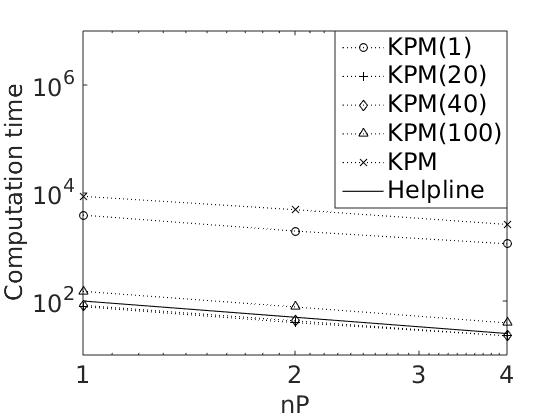
\includegraphics[width=\textwidth]{fig/u2para2}
                %\includegraphics[width=\textwidth]{test}
                \caption{function \texttt{P3}}
                \label{fig:speed2}
        \end{subfigure}
        \caption{Computation times for several methods with different number of processors. The helpline shows perfect speedup.}\label{fig:speed}

\end{figure}

\begin{table}[H]
\centering
\begin{tabular}{l | l l | l l}
%\textrhoticity Skriv påskeegg her!
%$\Pluto$
%\textrhoticity
%$\textrhoticity$
%\textpalhookvar
%$\textpalhookvar$
%\closedniomega $\closedniomega$
%\underwedge $\underwedge$
%$\pluto$ $\Pluto$
%$\libra$
$\neptune$ %$\Neptune$
%$\llcorner$
 &\texttt{P1} & & \texttt{P3} & \\
&\texttt{nP = 2} & \texttt{nP = 4} & \texttt{nP = 2} & \texttt{nP = 4} \\
\hline
KPM & 1.8556  &  3.5234 & 1.7702&    3.3193\\
KPM$(1)$ & 1.9858  &  3.3740 & 1.9725&    3.3924\\
KPM$(20)$ & 1.9883  &  3.4525 & 1.9756&    3.4547\\
KPM$(40)$ & 1.9619  &  3.6667 & 1.9352&   3.6642\\
KPM$(100)$ & 2.0083  &  3.8618 & 1.9437&    3.8362\\
\end{tabular}
\caption{Speedup for several cases of KPM.}
\label{tab:speedup}
\end{table}

\begin{table}[H]
\centering
\begin{tabular}{l | l l | l l}
&\texttt{P1} & & \texttt{P3} & \\
&\texttt{nP = 2} & \texttt{nP = 4} & \texttt{nP = 2} & \texttt{nP = 4} \\
\hline
KPM & 0.9278  &  0.8809 & 0.8851&    0.8298\\
KPM$(1)$ &  0.9929  &  0.8435 & 0.9862 &   0.8481\\
KPM$(20)$ & 0.9942  &  0.8631 & 0.9878&    0.8637\\
KPM$(40)$ & 0.9809  &  0.9167 & 0.9676&    0.9160\\
KPM$(100)$ & 1.0042  &  0.9655 & 0.9719&    0.9591\\
\end{tabular}
\caption{Parallel efficiency for several cases of KPM. }
\label{tab:eff}
\end{table}

From figure \ref{fig:speed} together with table \ref{tab:speedup} and \ref{tab:eff} we can observe the gain by using several processing units. Parallel efficiency and speedup is high for all cases of KPM tested here, it is definitely efficient to use several processing units on this type of problem. \\%All values of $n < m$ seams to give good parallel gain. \\

These experiments was only done with $m = k = 40$, this is because the experiments took a long time with this computer. I see no reason why parallel gain should change significantly with other $m$ or $k$. 

%%%%%%%%%%%%%%%%%%%%%%%%%%%%%%%%%%%%%%%%%%%%%%%%%%%%%%%%%%%%%%%%%%%%%%%%%%%%%%%%%%%%%%%%%%%%%%%%%%%%%%%%%%%%%%%%%%%%%%
\section{Comparison} \label{sec:compare}
%%%%%%%%%%%%%%%%%%%%%%%%%%%%%%%%%%%%%%%%%%%%%%%%%%%%%%%%%%%%%%%%%%%%%%%%%%%%%%%%%%%%%%%%%%%%%%%%%%%%%%%%%%%%%%%%%%%%%%
\begin{figure}[H]
        \centering
        \begin{subfigure}[b]{0.45\textwidth}
                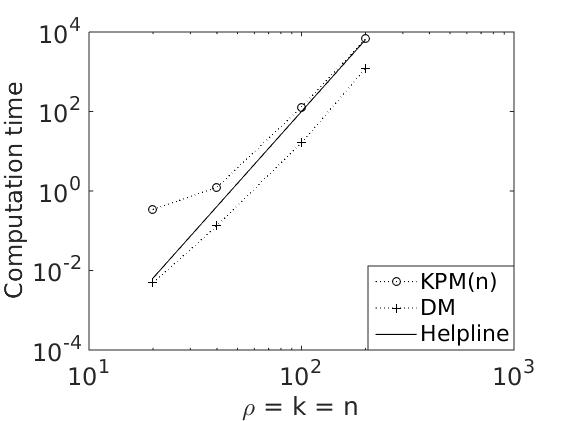
\includegraphics[width=\textwidth]{fig/comp2}
                \caption{function \texttt{P1}}
                \label{fig:c1comp1m}
        \end{subfigure}%
        ~
        \begin{subfigure}[b]{0.45\textwidth}
                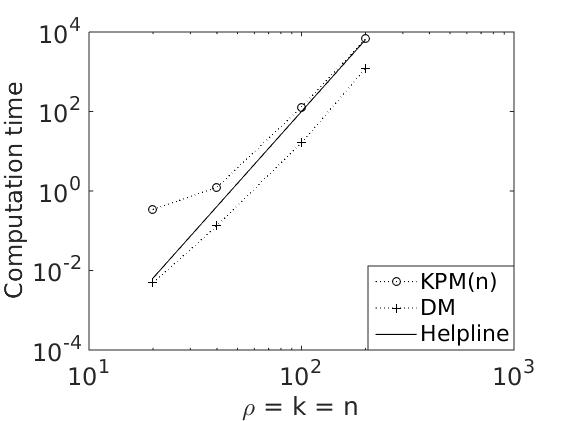
\includegraphics[width=\textwidth]{fig/comp2}
                \caption{function \texttt{P3}}
                \label{fig:c2comp2m}
        \end{subfigure}
        \caption{A plot of the computation times KPM$(n)$ and DM. We have used the values $n = \rho = k$, $\delta = 10^{-3}$ for the first point, and decreases with an order of magnitude for each additional point. Assume $\texttt{nP} = 4$ for KPM$(n)$ and $\texttt{nP} = 1$ for DM. These values are choosen to make KPM$(n)$ perform as efficiently as possible. The helpline increases with $\rho^6 = m^3$.}\label{fig:comp}
\end{figure}
From figure \ref{fig:comp} it is clear that DM is better in all cases simulated, but KPM$(n)$ is not far behind. We know from section \ref{sec:stimem} and\ref{sec:stimek} that one iteration of KPM$(n)$ is faster than DM, we therefore conclude that with enough processing units KPM$(\rho)$ would have been faster than DM. \\

The other important thing to note here is that computation time for KPM$(n)$ does not increase faster than for DM. It is difficult to say what would happen with larger $\rho$ or $k$, but they would probably follow the helpline.\\

The first point of KPM$(n)$ in both figures are very high compared to the trend, perhaps the problem size is to small to be used efficiently with several processing units. 
